\documentclass[a4paper,14pt]{extarticle}

\usepackage[utf8x]{inputenc}
\usepackage[T1,T2A]{fontenc}
\usepackage[russian]{babel}
\usepackage{hyperref}
\usepackage{indentfirst}
\usepackage{here}
\usepackage{array}
\usepackage{graphicx}
\usepackage{caption}
\usepackage{subcaption}
\usepackage{chngcntr}
\usepackage{amsmath}
\usepackage{amssymb}
\usepackage{pgfplots}
\usepackage{pgfplotstable}
\usepackage[left=2cm,right=2cm,top=2cm,bottom=2cm,bindingoffset=0cm]{geometry}
\usepackage{multicol}

\renewcommand{\le}{\ensuremath{\leqslant}}
\renewcommand{\leq}{\ensuremath{\leqslant}}
\renewcommand{\ge}{\ensuremath{\geqslant}}
\renewcommand{\geq}{\ensuremath{\geqslant}}
\renewcommand{\epsilon}{\ensuremath{\varepsilon}}
\renewcommand{\phi}{\ensuremath{\varphi}}

\counterwithin{figure}{section}
\counterwithin{equation}{section}
\counterwithin{table}{section}
\newcommand{\sign}[1][5cm]{\makebox[#1]{\hrulefill}} % Поля подписи и даты
\graphicspath{{pics/}} % Путь до папки с картинками
\captionsetup{justification=centering,margin=1cm}
\def\arraystretch{1.3}

\begin{document}

\begin{titlepage}
\begin{center}
	\textbf{Санкт-Петербургский Политехнический Университет \\Петра Великого}\\[0.3cm]
	\small Институт компьютерных наук и технологий \\[0.3cm]
	\small Кафедра компьютерных систем и программных технологий\\[4cm]
	
	\textbf{ОТЧЕТ}\\ \textbf{о лабораторной работе}\\[0.5cm]
	\textbf{<<Исследование частотных характеристик пассивных RC-цепей>>}\\[0.1cm]
	\textbf{Электротехника и Электроника}\\[10.5cm]
\end{center}

\begin{flushright}
	\begin{minipage}{0.60\textwidth}
		\begin{flushleft}
			\small \textbf{Работу выполнили студенты}\\[3mm]
			\small группа 23501/4 \hspace*{17mm} Дьячков В.В.\\[3mm]
			\small группа 23501/4 \hspace*{17mm} Ламтев А.Ю.\\[5mm]
			
			\small \textbf{Преподаватель}\\[5mm]
		 	\small \sign[3.5cm] \hspace*{8mm} к.т.н., доц. Кочетков Ю.Д.\\[0.5cm]
		\end{flushleft}
	\end{minipage}
\end{flushright}

\vfill

\begin{center}
	\small Санкт-Петербург\\
	\small \the\year
\end{center}
\end{titlepage}

\section{Цель работы}

Целью данной работы является экспериментальное исследование переходных процессов, происходящих в транзисторном ключе.

\section{Чертеж схемы исследуемого устройства}

\begin{figure}[H]
	\begin{center}
	\vspace{-0.5cm}
		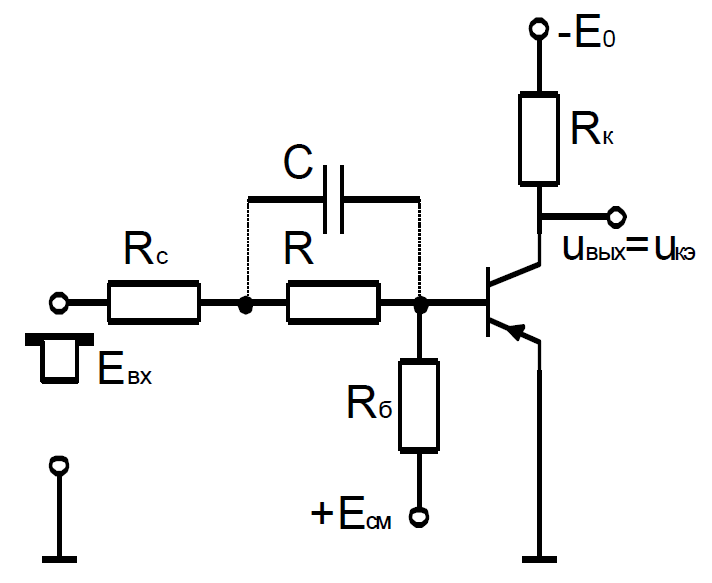
\includegraphics[width=7cm]{img/scheme}
		\caption{Схема транзисторного ключа с общим эмиттером}
		\label{figure:1}
	\vspace{-0.5cm}
	\end{center}
\end{figure}

\section{Исходные данные}

Транзистор МП25. Кремниевый транзистор с $p-n-p$ переходом.

\begin{table}[H]
	\begin{center}
	\caption{Исходные данные}
	\def\arraystretch{1.4}
		\begin{tabularx}{\textwidth}{|X|X|X|X|X|X|X|X|X|X|}
			\hline
			$E_0$ &
			$E_\text{см}$ &
			$I_\text{кн}$ &
			$S$ &
			$E_\text{вх}$ &
			$t_\text{и}$ &
			$R_c$ &
			$I_{к0 max}$ &
			$B$ &
			$f_\alpha$\\
			\hline
			В &
			В &
			мА &
			 &
			В &
			мкс &
			кОм &
			мкА &
			 &
			кГц\\
			\hline
			25 &
			5 &
			20 &
			3 &
			7 &
			10 &
			1 &
			75 &
			19 &
			200 \\
		    \hline	
		\end{tabularx}
		\label{tabular:1}
	\end{center}
\end{table}

\section{Теоретические расчёты}

\section{Экспериментально снятые зависимости}

\section{Выводы}

\end{document}
